
%%
\documentclass[12pt,twoside]{mitthesis}
\usepackage{lgrind}
\usepackage{graphicx}
\usepackage{enumitem}
\usepackage{arabtex}
\usepackage{utf8}
\usepackage{csquotes}

\usepackage{xltxtra}
\usepackage{fontspec}
\usepackage{polyglossia}
\setmainlanguage{english}
\setotherlanguage{urdu}
\setotherlanguage{arabic}
\newfontfamily\arabicfont[Script=Arabic,Scale=1, Path=font/]{Scheherazade-R.ttf}
\newfontfamily\urdufont[Script=Urdu,Scale=1, Path=font/]{jameel_noori_nastaleeq.ttf}

\usepackage{caption}
\pagestyle{plain}
\usepackage[backend=bibtex, sorting=none]{biblatex}
\addbibresource{bibliography.bib}
\usepackage{hyperref}
\hypersetup{pdftex,colorlinks=true,allcolors=blue}
\usepackage{hypcap}


\RequirePackage{filecontents}% write the data file
\begin{filecontents}{cycles.csv}
student,Muhammad Hassan Siddiqui
roll_no,MSCSF15M005
thesis_title,Urdu Text to Speech Synthesizer
supervisor_1,Dr. Muhammad Kamran Malik
\end{filecontents}

\usepackage{xparse}% mainly for \SplitList
\usepackage{pgfkeys}
\pgfkeys{/cycles/.is family, cycles,
  % allow arbitrary unknown keys and set with \pgfkeyssetvalue
  .unknown/.code={\pgfkeyssetvalue{\pgfkeyscurrentpath/\pgfkeyscurrentname}{#1}},
}
\newcommand\printcycle[1]{% print the key if it is defined and ??? otherwise
    \pgfkeysifdefined{/cycles/#1}{\pgfkeysvalueof{/cycles/#1}}{???}%
}

% split input line into key-value pair
\NewDocumentCommand{\AddCycle}{ >{\SplitList{,}} m }{%
  \AddCycleValue #1
}
% put a key-value pair into \pgfkeys{/cycles}
\newcommand\AddCycleValue[2]{\expandafter\pgfkeys\expandafter{/cycles,#1=#2}}

% \ReadCycles{filename} keys the keys in <filename> into \pgfkeys{/cycles}
\newread\cyclefile% file handler
\def\apar{\par}% \ifx\par won't work but \ifx\apar will
\newcommand\ReadCycles[1]{% read file into [\pgfkeys{/cycles}
  \openin\cyclefile=#1% open file for reading
  \loop\unless\ifeof\cyclefile% loop until end of file
    \read\cyclefile to \cycleline% read line from file
    \ifx\cycleline\apar% test for \par
    \else%
      \ifx\cycleline\empty\relax% skip over empty lines/comments
      \else\expandafter\AddCycle\expandafter{\cycleline}%
      \fi%
    \fi%
  \repeat% end of file reading loop
  \closein\cyclefile% close input file
}
\ReadCycles{cycles.csv}% read the file


\begin{document}
\setcode{utf8}



\begin{center}
\Large{\textbf{\printcycle{thesis_title}}}

\end{center}
\bigskip

\begin{center}


%\begin{figure}[h]

\includegraphics[width=6cm, height=6cm]{images/logo.PNG}
%\caption{}
%\end{figure}
\end{center}

\begin{center}


    By

\bigskip
\large{\textbf{\printcycle{student}}}

\bigskip
\large{\printcycle{roll_no}}

\bigskip
Supervised by

\bigskip
\large{\textbf{\printcycle{supervisor_1}}}


\bigskip
Assistant Professor, PUCIT

\bigskip
(June, 2018)

\bigskip
Punjab University College of Information Technology,

\bigskip
University of the Punjab, Lahore, Pakistan.

\end{center}

\newpage
\begin{center}
\Large{\textbf{\printcycle{thesis_title}}}



A THESIS

SUBMITTED IN PARTIAL FULFILLMENT OF THE REQUIREMENTS FOR THE

DEGREE OF

MASTER OF PHILOSOPHY

IN

COMPUTER SCIENCE

\bigskip

    By

\large{\textbf{\printcycle{student}}}

\large{\printcycle{roll_no}}

\bigskip
Supervised by

\large{\textbf{\printcycle{supervisor_1}}}

Assistant Professor, PUCIT

%\bigskip
%Co-Supervised by

%\large{\textbf{Dr.Zubair Nawaz}}

%Assistant Professor, PUCIT

\bigskip
(June, 2018)

\bigskip
Punjab University College of Information Technology,

\bigskip
University of the Punjab, Lahore, Pakistan.

\end{center}
\bigskip


%\author{Lucien William Van }
%\supervisor{William J. Dally}{Associate Professor}

%\department{Department of Electrical Engineering and Computer Science}
%\begin{figure}[h]
%\centering
%
\includegraphics[width=4cm, height=4cm]{a.PNG}
%\end{figure}


%\degree{Bachelor of Science in Computer Science and Engineering}

%\degreemonth{June}
%\degreeyear{1990}
%\thesisdate{May 18, 1990}


%\chairman{Arthur C. Smith}{Chairman, Department Committee on %Graduate Theses}

%\maketitle

%\cleardoublepage
%\setcounter{savepage}{\thepage}

%\begin{abstractpage}


%% ************************** Thesis Abstract *****************************
% Use `abstract' as an option in the document class to print only the titlepage and the abstract.
\begin{abstract}
This is where you write your abstract ...
\end{abstract}

%\end{abstractpage}


%\cleardoublepage

%\section*{Acknowledgments}

%This is the acknowledgements section.  You should replace this with your
%own acknowledgements.

%%%%%%%%%%%%%%%%%%%%%%%%%%%%%%%%%%%%%%%%%%%%%%%%%%%%%%%%%%%%%%%%%%%%%%
% -*-latex-*-


\begin{center}
    

\large{\textbf{Evaluation of M. Phil. Thesis}}
\end{center}

We have evaluated the M. Phil. thesis titled
\begin{center}
\textbf{ \printcycle{thesis_title}}
\end{center}

Submitted by Mr. \textbf{\printcycle{student}}, \textbf{\printcycle{roll_no}}, session 2015-2018 in partial fulfillment of the M. Phil. degree in Computer Science. We have also assessed the candidate through viva-voice.

We are satisfied with the thesis and performance of the candidate in the examination and are of the opinion that she fulfills the requirements as set in the rules and regulations for the M.Phil. degree in Computer Science at the University of the Punjab.

\bigskip
\bigskip
 \textbf{Thesis Supervisor}:	\hfill \printcycle{supervisor_1}

\hfill Assistant Professor

\hfill Punjab University College of Information Technology

\hfill University of the Punjab, Lahore



\bigskip

\bigskip
\textbf{Principal of the College}:  \hfill Dr. Syed Mansoor Sarwar
Principal, 

\hfill Punjab University College of Information Technology

\hfill University of the Punjab, Lahore

% % -*- Mode:TeX -*-
%
% Some departments (e.g. Chemistry) require an additional cover page
% with signatures of the thesis committee.  Please check with your
% thesis advisor or other appropriate person to determine if such a 
% page is required for your thesis.  
%
% If you choose not to use the "titlepage" environment, a \newpage
% commands, and several \vspace{\fill} commands may be necessary to
% achieve the required spacing.  The \signature command is defined in
% the "mitthesis" class
%
% The following sample appears courtesy of Ben Kaduk <kaduk@mit.edu> and
% was used in his June 2012 doctoral thesis in Chemistry. 

\begin{titlepage}
\begin{large}
This doctoral thesis has been examined by a Committee of the Department
of Chemistry as follows:

\signature{Professor Jianshu Cao}{Chairman, Thesis Committee \\
   Professor of Chemistry}

\signature{Professor Troy Van Voorhis}{Thesis Supervisor \\
   Associate Professor of Chemistry}

\signature{Professor Robert W. Field}{Member, Thesis Committee \\
   Haslam and Dewey Professor of Chemistry}
\end{large}
\end{titlepage}


%Publication rights, dedication(:P), Abstract, acknowledgements
%\documentclass[12pt]{article}

%\usepackage{amsmath}    % need for subequations
%\usepackage{graphicx}   % need for figures
%\usepackage{verbatim}   % useful for program listings
%\usepackage{color}      % use if color is used in text
%\usepackage{subfigure}  % use for side-by-side figures
%\usepackage{hyperref}   % use for hypertext links, including those to external  documents and URLs
%\usepackage{latexsym}


%\oddsidemargin -0.5in 
%\evensidemargin -0.5in 
%\textwidth 7.5in 
%\headheight -0.5in 
%\topmargin 0in

%\begin{comment}
%\pagestyle{empty} % use if page numbers not wanted
%\end{comment}
% above is the preamble
%\begin{document}

\begin{center}
\textbf{ UNIVERSITY OF THE PUNJAB } % \\ = new line 
\end{center}


\subsection*{} 
\vspace{7mm}
Author: \hspace{10mm} % for space or use \quad
\textbf{\printcycle{student}}  \\
Title: \hspace{13mm}
\textbf{ \printcycle{thesis_title}} \\ 
Department: \quad
\textbf{Punjab University College of Information Technology}\\ 
Degree: \hspace{7mm}
\textbf{\quad M. Phil. (Computer Science)}\\ 


\subsection*{}
Permission is herewith granted to University of the Punjab to circulate and to have copied for non-commercial purposes, at its discretion, the above title, upon the request of individuals or institutions. 
\\ \\ 
\begin{flushright}
\textbf{Signature of the Author}
\end{flushright}
 
 %\bigskip


\subsection*{}
%\vspace{15mm}
\small{THE AUTHORS RESERVE OTHER PUBLICATION RIGHTS, AND NEITHER THE THESIS NOR EXTENSIVE EXTRACTS FROM IT MAY BE PRINTED OR OTHERWISE REPRODUCED WITHOUT THE AUTHOR’S WRITTEN PERMISSION.\\
THE AUTHORS ATTEST THAT PERMISSION HAS BEEN OBTAINED FOR THE USE OF ANY COPYRIGHTED MATERIAL APPEARING IN THIS THESIS (OTHER THAN BRIEF EXCERTS REQUIRING ONLY PROPER ACKNOWLEDGEMENT IN SCHOLARLY WRITING) AND THAT ALL SUCH USE IS CLEARLY ACKNOWLEDGED.}






\vspace*{\fill}
{\centering\huge\bfseries Dedicated to\par}
\bigskip
%\noindent Some text here...
\vspace*{\fill}



{\LARGE\textbf {Abstract}} \\ % \\ = new line
The process of transformation of data from textual form into voice output is called speech synthesis. The type of system which plays out this assignment is known as a text to speech (TTS) system or sometimes as speech synthesizer. The synthesized speech sometimes referred as artificial speech. This system can assist individuals with various handicaps like visual weakness in their day by day undertakings and furthermore help in inter language correspondence. These systems are being used in screen reading software, games, animations, machine to machine communication and may other applications. Artificial speech can be synthesized by concatenation of small segments of speech series of words. Formant synthesis and unit selection synthesis are based on this types of synthesis system. Another popular technique which is being used in most recent couple of years is statistical parametric speech synthesis. This technique when used with Hidden Markov (HMM) or Deep Neural Networks (DNN) gives extremely promising results.

In this paper, development of statistical parametric speech synthesis system using Festival TTS for Urdu is discussed. HMM based TTS system is developed using 70 minutes of speech data. This paper divides complete process of speech synthesis in two sub processes i.e. text preprocessing and speech synthesis. Text preprocessor system identifies and processes special characters, numbers (Arabic numerals, floating point and whole numbers), time and dates text in input data. Speech synthesis process takes processed input and converts it into corresponding voice. In this process, Lexicon and letter to sound rules of Hindi are used. In the last step, performance of system evaluated using Diagnostic Rhyme Test (DRT), Modified Diagnostic Rhyme Test (M-DRT), Naturalness Test, Intelligibility Test and Usability Test.


\\ \\ \\
\textbf{Keywords:}
Text to Speech, Urdu Text Preprocessor, Hidden Markov model, Festival, Festvox

{\Large{\textbf {Acknowledgements}}} \\ \\% \\ = new line
Computational modeling is branch of computer science which deals with multiple disciplines. It assists other domains in understanding complex systems and phenomena by providing theory, tools and technology to model and simulate related systems and phenomena. In complex systems, behavior of an individual can have butterfly effect and can become root cause of an emergent phenomenon. Interaction of drivers with each other and surrounding environment forms the dynamics of traffic flow. Hence global effects of a traffic flow depend upon behavior of a single driver. In this research.


\pagestyle{plain}


  % -*- Mode:TeX -*-
%% This file simply contains the commands that actually generate the table of
%% contents and lists of figures and tables.  You can omit any or all of
%% these files by simply taking out the appropriate command.  For more
%% information on these files, see appendix C.3.3 of the LaTeX manual. 
\tableofcontents
\newpage
\listoffigures
\newpage
\listoftables


\chapter{Introduction}

\section{Speech Synthesis}

Speech is the most important medium of conveying opinions and expressing feelings and thoughts.
Human convert their thoughts into speech by using words, phrases and sentences in order to communicate \cite{mumtaz2016break}. 
Speech is produced when air is exhaled by the lungs and vibrations are produced by air, these vibrations get a 
proper waveform shape by glottal cords and vocal tract. Text to Speech synthesis is the process of conversion of raw text into 
speech signals. It works by concatenation of small segments of recorded speech called phonemes \cite{khilari2015review}. Speech data is obtained by first recording natural speech by using some type of recording systems and is converted to digital form. The digital data is sampled and stored in computer, after that passed back to analog signals and is converted back to speech \cite{greene1986perception}. 

Text to speech systems are becomming important as they can be used in machines to effectively transmit
information to human using artificial speech as information exchange through computers has become the integral part of new
era. Visually impaired people usually suffer while using computer technology when there is no assistant or
computer is not enough interactive which makes text to speech systems necessity of modern life. These
systems increase the degree to which blind people can interact with sighted people \cite{klatt1987review} and could boost up
their hope to survive in this world gracefully \cite{aida2010main}. Many applications of speech synthesis are emerging such as 
machines that read for blinds, aids for handicaps, computers that interact with user through speech. 
For all these applications a text to speech that convert text to speech are used \cite{klatt1982klattalk}.

The TTS system comprises of two main stages. One is called Natural language Processing (NLP) and
other is called Speech Synthesis (SS). This is shown in figure \ref{fig:TTS Block Diagram}.

\begin{figure}[hp]
  \centering
  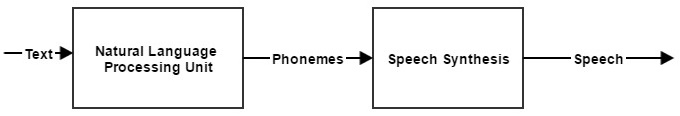
\includegraphics[width=\linewidth]{images/tts_bd.jpg}
  \caption{TTS Block Diagram}
  \label{fig:TTS Block Diagram}
\end{figure}

In NLP unit, text is first converted into string of letters and then word boundaries are marked by
tokenizer. This is called normalization of text. Normalized data is then converted into phonetic strings
with the help of letter to sound rules after which syllabifier marks syllable boundaries. Sound change
rules are applied on the syllabified data. Language modeling techniques are also applied for finding
context in which a specific word is used. As human has tendency to recognize basic rules for his native
language, it is easy to judge context of a word in a sentence and what should be correct pronunciation of
that word with respect to its context. For example, it can be guessed easily that \enquote{\texturdu{پل}} in a sentence is used
for \texturdu{پل} (moment) or \texturdu{پل} (bridge) for any native speaker of Urdu. But for computer, we need to mark context of each word according to data. 
Last stage of NLP is stress intonation marker which adds stress and intonation to the text. Speech Synthesis unit converts symbolic information
received from NLP unit into audible speech with the help of different Digital Signal Processing
techniques. The quality of speech synthesis system is detected by naturalness and intelligibility of the speech.

In digital world, there are some people who can read and understand different languages and some
who can’t understand languages except their own language. Speech to text conversion system can
also provide a facility to exchange information between people speaking different languages \cite{khilari2015review}. 
TTS systems are also needed to reduce the extinction of
minority languages. As minority languages of the world are facing challenge of extinction
considerable efforts are going on from last few years for their survival. Fon language is spoken in
Republic of Benin and some other regions of Africa and it is also facing challenge of extinction \cite{dagba2014text}. 
The Xitsonga is spoken in more than three African countries.
TTS system of such languages will help lot of people of different literacy level \cite{baloyi2012text}.
Urdu is national language of Pakistan and it is spoken by more than 100 million people across the world \cite{top_30_languages}.
A Text-to-Speech (TTS) system for Urdu will be very helping for visually impaired, handicapped and illiterate people.

For human, the task of speech synthesis is not difficult one as they have basic knowledge of their
language but for computer some other method has to be implemented for this task. When we talk about TTS systems speech types
and procedure for synthesis, strategies or modules used to develop systems etc. are important to
consider. Different types of speech exist such as isolated word (process single word at a time),
connected words (isolated words but separated with least gap), continuous speech (permit client
to talk while computer is processing content) and spontaneous speech (deals with variety of words
that are used rarely) as well as two types of speaker model were presented independent and
dependent of clients or speaker specifications. Vocabulary is also characterized according to size
such as small vocabulary, medium vocabulary, large vocabulary, very large vocabulary and out-of-vocabulary.
Below are the major speech generation techniques.

\section{Types of Speech Synthesis}
For the process of speech synthesis, three types of techniques are used.

\subsection{Formant Synthesis}
In Formant Synthesis, speech waveform is generated using concatenation of sine wave with the help of some algorithms to model a source of sound \cite{format_synthesis}. All speech parameters are changed periodically in order to get speech waveform. Some set of rules are also used to generate speech due to which this technique is also called rule based speech synthesis. But it is very difficult to accurately describe the process of speech generation in set of rules therefor the speech generated by this technique is not very natural but intelligible.

\subsection{Concatenative Synthesis}
In concatenative synthesis, small units are selected from carrier sentences which are joined to form
speech of complete sentence. These small units are called phonemes. These are the units which
collectively describe correct pronunciation of a word. This process is easy as compared to previous one
as number of such phonemes are limited for any language. For English, there are 44 such phonemes.
Similarly in Urdu, there are 44 consonants, 8 long vowels, 7 long nasal vowels, 3 short vowels and many
diphthongs \cite{saleem2002urdu}. This reduce distortion but it can decrease the naturalness.
That’s why the derived synthetic speech may not resemble the donor speaker in training database \cite{huang1996whistler}.

\subsection{Statistical Parametric Speech Synthesis}
Statistical parametric speech synthesis is another approach which uses parameters to describe
speech. In this technique, model is learned from speech data. This technique works better than
concatenative technique \cite{merritt2013investigating}. 

\section{Quality of Speech Synthesis System}
Intelligibility and naturalness is the measure of quality of the synthesized speech \cite{swetha2013text}. 
There are lots of experimentation over naturalness of voice as a result of TTS
systems. In today’s world, different segments are recorded and then concatenated for completing a
message. A collection of speech words is collected and maintained in database by using a reader
who reads large series of text. In these kind of systems, to maintain the consistency the speaker
speaks in a single style and keep in mind the distance from microphone and other factors to avoid
the inconsistency. This type of TTS system is not required at all as the need is to have a system
which can be expressive and convey message with proper expressions and styles. Work is
performed to build a system that can convey the message according to the needs of the users. A
single style of communication can lead towards wrong messages and can cause other problems of
misunderstandings. For example, it is not appropriate to convey a good news and bad news in a same
style and manner. Similarly, it is not acceptable to ask a question in neutral way of communication \cite{eide2004corpus}.
Multiple techniques like linear regression and neural networks were applied to get the improved results. Concatenation techniques are applied to get fully
expressive and stylish messages for end users. By using concatenation technique, users can
customize, add styles and expression through provided Speech Synthesis Markup Language (SSML) \cite{eide2004corpus}. 
Timing of events in speech is also important as timing of events in
speech signals are affected by some contextual factors like phone identity factors. These factors
make it difficult to control timing of events \cite{tokuda2000speech}. There are some approaches which have been proposed
to control timing of events like linear regression \cite{kaiki1992linguistic} and tree regression \cite{riley1992tree}. 
A new technique is proposed in \cite{tokuda2000speech} where timing of events is
controlled by multi-dimensional Gaussian distribution based Hidden Markov model.

\section{Architecture}
Text to speech is a way of communication and transferring information using words and styles of
speaking \cite{eide2004corpus}. It has two processes which are text processing and speech
generation. In text processing given input text is processed so that to get appropriate chain of
phonemic units. Speech generator takes these units as inputs and convert them into synthetic
speech by selection of a unit from large corpus TTS system for small database is easier to
implement but not in good quality \cite{black2007statistical, zen2007hmm, raj2007text}.
Different researchers and developers used different strategies and architecture to develop TTS system. In \cite{kabir2002natural}, raw text is converted into intelligible speech signals by following two sub processes called High-level synthesis and Low-level synthesis. High-level
synthesis converts text into phonetic strings and Low-level synthesis converts these strings into
speech signals \cite{kabir2002natural}. In \cite{hussain2005phonological}, TTS system is divided in three modules.

\begin{enumerate}
  \item Natural language Processing
  \item Text Parameterization
  \item Speech Synthesis
\end{enumerate}

Natural Language processing unit converts text into phonetic strings. The second and
third stages use these phonetic strings and convert them into speech signals. This is shown in figure \ref{fig:Architecture of TTS}.

\begin{figure}
  \centering
  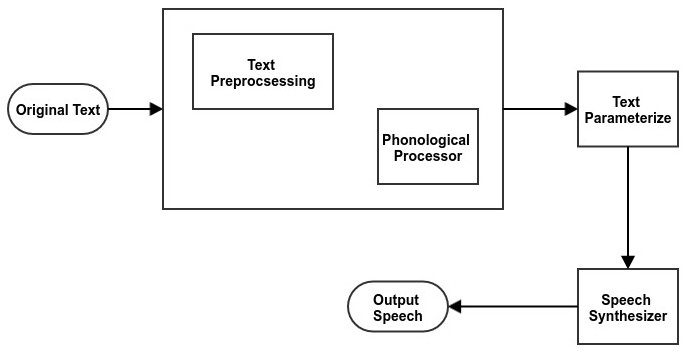
\includegraphics[width=\linewidth, height=7cm,keepaspectratio]{images/tts_block_dg.jpg}
  \caption{Architecture of TTS}
  \label{fig:Architecture of TTS}
\end{figure}

\\
In \cite{liberman1992text}, TTS system is implemented by following four modules in
sequence.

\begin{enumerate}
  \item Text Analysis
  \item Word Pronunciation
  \item Phonetic Interpretation
  \item Speech Signal Generation
\end{enumerate}

In text analysis, the input text is segmented into sentences and later on dividied into words.
These words are then categorized according to their syntactic and contextual meaning. The
numbers and abbreviations are also processed in this step. In word pronunciation process, words
are represented by respective phonetic notations by using word pronunciation dictionary. In
phonetic interpretation the duration of phonetic segments, pitch, accents are assigned. Signal
generation component of TTS system takes output from all above processes and generate a signal
of speech using a function. In \cite{urdu_text_preprocessing}, text-to-Speech system is divided in
two parts. One is called Natural Language Processing unit and other is called Speech Synthesis
unit. Natural Language Processing unit preprocess text and converts it into phonetic strings. These
phonetic strings are then marked by stress marker and passed to speech synthesis unit which
converts it into speech signals.
\chapter{Related Work}

Text to speech synthesis is not a new field and people have been working on this field before electronic
signal processing techniques. In beginning, people tried to build machines with mechanical devices which were used to
create human sound. After the development of computers, better systems were built using different
techniques. In \cite{swetha2013text}, basic speech synthesizing technique are discussed 
which works by concatenation of small recorded speech segments called phonemes to form
complete speech. Each word is first divided into syllables and then corresponding voice signal for each syllable
is concatenated in order to get pronunciation for whole word. This concatenated word has some
delay between pronunciations of each syllable which is removed and as a result of which final
pronunciation of that word is obtained. Problems like Text Preprocessing, Pronunciation and
Prosody make this system difficult. In Text Preprocessing, digits and abbreviations are converted to full
words. Other problem is the guessing correct pronunciation of a word. For example, word “lives” has
different pronunciation in “He lives in Lahore” and “He saved two lives”. To create naturalness in
sound, stress and intonation are applied to the input text which is also a very complex task. A TTS system for Azerbhaijani 
language is developed using concatenative synthesis in \cite{aida2010main} where small recordings 
were concatenated to make speech waveform.

Two sub parts of text-to-speech system text analysis and word pronunciation were discussed in \cite{liberman1992text}. 
TTS system is divided in 4 sub parts: text analysis, word pronunciation, phonetic interpretation and signal
generation. Text analysis step includes division of text into sentences, words, phrases and expansion of abbreviations etc.
Text analysis is required to get correct context and pronunciation of each word in a sentence. In text analysis, 
sentence division and parts of speech tagging is done by using heuristic solutions \cite{riley1989some}
and dynamic programming respectively. For word pronunciation, dictionary based approach was used for about 99.9\%
words and for 0.1\% words, letter to sound rules were followed. 

A technique based on letter to sound rules is also developed in \cite{elovitz1976automatic}. Total 329 letter to sound rules have been created. These rules take text as input and translate it into phonetic alphabet which in turn converted to synthetic sound. This system produces about 97\% correct pronunciation of phonemes. The paper also describes software and hardware requirements and overall performance statistics of this system. The dataset is developed by extracting 50,000 words from standard corpus, Corpus of present-day edited American English i.e. Brown corpus \cite{ku1967computational}. The system gave accuracy of about 93\%. A more improved system was proposed in \cite{carlson1982multi, klatt1982klattalk}. In \cite{klatt1982klattalk}, a TTS system is developed for English and simple numerical and algebraic expressions. The system is rule based system having 500 letter to sound rules. However, it can use pronunciation dictionary of 1500 words for exceptions. The system interface provides facility of selection of voice types (Male or Female). The word boundaries and probable position of phrases and clauses is analyzed by syntactic analyzer. The phonemes of word are then passed to synthetic speech synthesizer that converts phoneme to sound by following extensive set of rules and rules for consonant-vowel transitions. The whole process is divided in two sub processes, text analysis which is conversion of text to corresponding linguistic representation that comprises of phoneme, stress and boundaries and positions of respective vowel or consonant and durational phenomena such as pauses, interaction between segments \cite{klatt1979synthesis} and speech synthesis in which sequence of phonemes are converted to speech sound with the help of some set of rules. The abbreviations in input data are converted to their respective text and if dictionary does not have their respective words, the abbreviation is pronounced as a word. After preprocessing, the words are exposed to letter to sound rules. If an unstressed function appears in text and there is no rule for it then it is passed to pronunciation dictionary. The results show that about 95\% rules were successful when executed. The syntactic analyzer then determines the structure of sentence according to its pauses and boundaries. The phoneme to speech rules are divided into two components, phonological that provide information of stress and rhythm and duration of words in a sentence. All these outputs are then passed to synthesizer that produces synthetic sound. Synthesizer is simple version of synthesizer proposed in \cite{klatt1980software}.

In \cite{carlson1982multi}, a text to speech system is presented which require some hardware resources as well with the enhancements in microprocessor, 
memory and signal processor technology. This TTS system can be put into portable form and can be used anywhere with different systems. A higher level language is
developed in laboratory that can be easily used for linguistic processes. These enhancements and developments in hardware
and software level made transforming of text to speech at 250 wpm rate. This combination of hardware and software is tested
against several applications used for handicaps. The main purpose of this system is to make a framework that will
be used for conversion of any language text to speech. 

In \cite{huang1996whistler}, Whistler which is a Text-to-Speech engine is developed by using prosody and
concatenative speech parameters that were extracted through use of probabilistic learning methods. Whistler engine produce
speech which appears to be very much real. This system can also help to build TTS system for other languages.

A formant and concatenative synthesis is developed in \cite{huang1997recent}
where small segments of phonemes were concatenated to form whole speech. A training database was used which 
contains about 6,000 phonetically balanced sentences recorded in natural style. The technologies used in whistler can considerably facilitate the
process of creating generic TTS system for new speech style. This engine supports Microsoft Speech API \cite{ms_speech_api} and requires less than 3 MB memory.

In \cite{hunt1996unit}, linear regression and unit selection 
based speech synthesis is designed using ATR Japanese database. In this algorithm, raw text is converted to phonetic strings and against each phoneme, best candidate unit from a huge database of speech units is selected with \textit{Viterbi} search. By concatenating these units, target waveform is generated. The units in database can be considered as state transition network where each unit represents a different state. The cost of the system depends on target cost and cost of the concatenation of units. Each phoneme and unit is represented by a multi-dimensional feature vector. The target cost is measured by the weighted difference of target and candidate feature vector. Similarly, concatenation cost is also weighted sum of sub-cost of concatenation. Cost function can be trained in two different ways. In Weight Space Search method, units are searched with \textit{Viterbi} and distance between constructed waveform and
natural waveform is minimized. In Regression Training, linear regression is used to choose best unit from the list of all possible
units for a given phoneme. 

Statistical parametric speech synthesis is another approach which uses parameters to describe
speech \cite{king2010beginners}. This technique works better than
concatenative technique on smaller data. On larger data, concatenative synthesis can produce better quality speech. In this technique, Hidden Markov model (HMM) or model firmly related to HMM are used for training model over given data. HMM based statistical parametric speech synthesis has gained popularity because of its ability to produces high quality speech automatically with parametric flexibility, less data and resources \cite{black2007statistical}.

A multi-dimensional Gaussian distribution based Hidden Markov model based statistical parametric speech synthesis system was developed in
\cite{yoshimura1998duration}.  In this technique, decision tree based context clustering is used for duration models clustering. The contextual factors are also considered with phone identity factors. Mel-cepstral coefficients are
calculated and model is trained by these coefficients. State of the context dependent HMMs is clustered using decision tree based
context clustering technique \cite{odellj.j1995}. In state duration modeling, multi-dimensional Gaussian distributions are
used to model Hidden Markov model. Duration models are clustered after estimation using decision tree based clustering techniques. 
By traversing decision tree, all contexts can be searched. Contextual factors which effects timing of
events in speech are also taken into account and resultant speech shows that it has good quality and natural timing. For testing
of the system, 450 sentences of Japanese are used for training of system. Sampling of speech signal is done at 16 kHz. Feature
vector is composed of 25 mel-cepstral coefficients. There were 3030 states and 2984 distributions in output of the system.
The listening tests show that synthesized speech has good quality and it has natural timing even if speaking rate is changed to
some degree.

A similar system is designed in \cite{tokuda2000speech} using HMM and evaluated by taking input
from Japanese database. The parameters in this system are generated with Hidden
Markov model. The state sequence fully or partially is hidden due to which iterations are performed for parameter generation and
forward-backward algorithm is used for the situation where state sequence is provided. This algorithm, from multi-mixture HMMs,
can generate clear formant structure.

A HMM and unit selection based system is proposed in \cite{tokuda2002hmm} where model is trained with speech database after which excitation and spectral parameters are extracted. These extracted parameters are modeled by context dependent HMMs. To find
accurate model parameters, decision tree based context clustering is used. The parameters are then used to generate speech
signals. These parameters can be used to control speech characteristics. In \cite{harashima2006review}, HMM and rule based approaches are applied 
on voices taken from e-learning courses and online lessons for dataset creation and tested by
generating voices and given as input to students to interpret it.

Corpus based approach for Expressive Prosody Modeling is applied in \cite{eide2004corpus} where manually produced dataset was used. To evaluate the synthesized
speech and expression, the output is given for testing to 32 native English speakers. Test is performed with different types of sentences like bad news, good news and for yes/no and the accuracies we get are 70.2\%, 80.3\% and 84\% respectively.

% Tones and Break Indices ToBI are discussed on American English in \cite{pitrelli2004tobi}. Majorly
% bi-gram and tri-gram were used to predict the occurrences of particular word or letter. Analysis
% was performed by multiple techniques. The corpus was divided into following five yes-no
% questions, either-or questions, other questions (hereafter, “wh-questions”), exclamations, and other
% declarative sentences categories for the analysis purpose. Analysis by word frequency count
% produced not good results and the reason was that the data was of variant types. The results show
% that professional speakers produces better and informative prosodic events as compared to
% ordinary speakers.

HMM based approach is used in \cite{baloyi2012text} to construct a speech synthesizer for Xitsonga which is an African language. The dataset used here consists of phone set of consonants and vowels. These sets are used to prepare a set of letter to sound rules to be used in speech synthesis system. The main tool used for speech synthesis is HTS toolkit \cite{hts_2.2} with other software that support to setup complete environment for text-to-speech conversion. The technique used in this study is Hidden Markov model because the statistical parametric speech synthesis based on HMM can be used to synthesize speech waveform without requiring huge dataset for training. The system received acceptability of 92.3\%. 

TTS system for Fon language is designed in \cite{dagba2014text} using Multisyn algorithm \cite{clark2007multisyn} which consists of Natural Language Processing (NLP) and Digital Signal Processing (DSP) modules. NLP consists of segmentation, Letter-to-Sound conversion and back-off rules module. Back-off rules are applied when input text contains some characters that are not in us know characters. DSP module than choose required unit from database of units are concatenate them to form complete speech signals.

In \cite{ganai2016text}, hybrid text to speech converter is developed by
concatenating benefits of HMM based TTS system and waveform based TTS system. For developing it, an audio phoneme library is used. The main
edge of developed system over other is that it produced more human like voice/speech. The experiments were taking in
matlab and a phoneme library is developed that consists of audio files and dictionary of words with their phoneme. Sentence is
taken as input then model parsed it into words. The system analyzes each word, gets its phoneme and combines all phonemes
and plays the sound. Waveform for each sound is also presented. This sub-ban speech synthesized approach is obtained by
this combination of models that improved the quality of synthesized speech. The current model is not good enough, in future
system will be improved to get better controls.

A speech synthesis system is introduced in \cite{donovan1995improvements} which uses context-dependent Hidden Markov Model for defining set of subphone units. This system uses context-dependent HMM for defining set of subphone units. These subphone units are then used in concatenation synthesizer. The training data is one hour recorded speech which is used for getting required parameters. TD-PSOLA waveform concatenation synthesizer is then used to generate pronunciation using these parameters. The synthesized speech imitates the voice of the speaker used to record the preparing database. This system uses automatic statistical processes to extract segments of speech from large speech carpus. Desired sentence is produced by concatenation of small segments of speech. Hidden Markov model is trained and used for segmentation of speech database into HMM-state-sized units. A decision tree is constructed by using phonetic context labels which is used for clustering of the training speech into acoustically self-comparable grouped states. This process helps to find most important context effects. The string to be converted into speech is first converted into sequence of phonetic strings which then with the help of decision tree is converted to speech segments which are used to generate final speech signals. Modified Rhyme Tests \cite{house1965articulation} were used to compare system with other. Six listeners were used with each give an answer sheet, and they have to mark word from list of provided words which is played during test. The MRT error rate for test was 5.0\% and standard error rate was 0.47\%. Hidden Markov model is used for training of the model. The dataset used for training of model is recorded speech. Four datasets are used in which are termed as M2, M3, F1 and F2 where M stands for male and F stands for female. Six listeners evaluate output produced by model. Error rate is used as measure of performance. The MRT error rate for test was 5.0\% and standard error rate was 0.47\%. In future, segment selection algorithm used in the system can be improved where segments in each state would be available in speech synthesis process. Dynamic programming can be used to find optimal segment sequence.

\cite{masuko1996speech} present a TTS system which is based on HMM which comprises dynamic features. The statistical parametric speech synthesis system can change voice characteristics of speech by speaker adaptation technique \cite{tamura1998speaker} and speaker interpolation technique \cite{yoshimura2001speaker}. The Hidden Markov Model statistical parametric text-to-speech system can model speech parameters like spectrum or excitation with the help of context-dependent HMM and construct speech signals. Version 2.0 of already build HMM based text to speech system (HTS) toolkit is presented in \cite{zen2007hmm}. HMM based speech synthesis system can be used to build speech synthesis system with small dataset for training \cite{huang2001spoken} but the quality of that speech will not be equal to recorded speech. 

% In \cite{merritt2013investigating}, author discussed shortcomings of Hidden Markov model and majorly focused on the findings that HMM based TTS system are not better than simple concatenative TTS systems. Experiments performed and then through pairwise listening test, the HMM based system is evaluated. Based on the responses of qualities, model molded to tackle further situational problems. In figure \ref{fig:Merritt_tts}, architecture of this system is shown.
% \begin{center}
% 	\begin{figure}[hbtp]
% 		\centering
% 		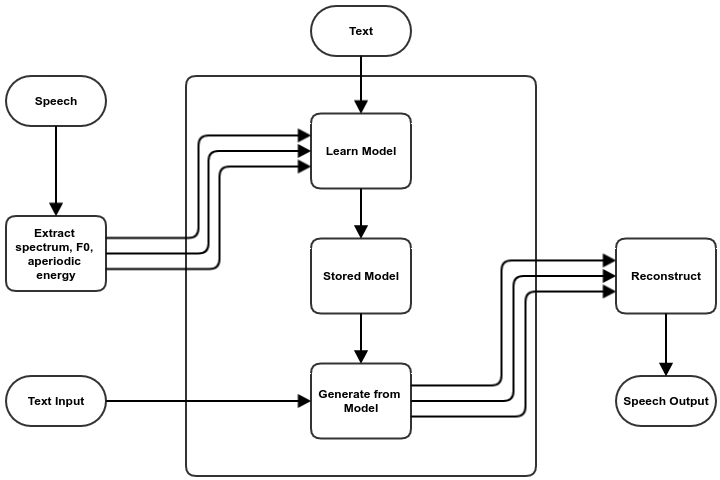
\includegraphics[width=\linewidth]{images/Merritt_tts.png}
% 		\caption{TTS System Architecture using HMM speech synthesiser}
% 		\label{fig:Merritt_tts}
% 	\end{figure}
% \end{center}

% Experiments show that when variance is too high then smoothing has a beneficial effect as it
% reduces the variance and bring the points closer to the natural one. For future, needs to work over spectral envelope over-smoothness, averaging across multiple tokens of similar speech sounds, model boundary discontinuities in the trajectory and
% inconsistencies between the different speech parameter streams \cite{merritt2013investigating}.

A more advance technique is Neural Networks based technique as it works better than Hidden Markov model based technique. Time domain Neural Networks with database containing sounds of words called phonemes is used in \cite{karaali1998text}. The basic flow of the system involves speech recording, speech labeling, voice coder and input processing using Time Delay Neural Network. The figure \ref{fig:Time Domain Neural Networks based TTS System} shows the block diagram of system.

\begin{center}
	\begin{figure}[hbtp]
		\centering
		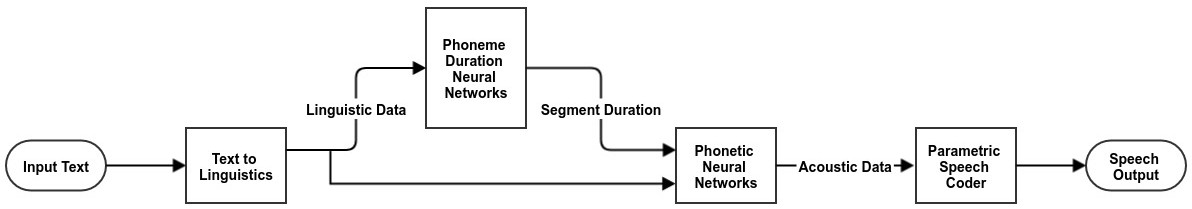
\includegraphics[width=\linewidth]{images/time_domain_neural_network.jpg}
		\caption{Time Domain Neural Networks based TTS System}
		\label{fig:Time Domain Neural Networks based TTS System}
	\end{figure}
\end{center}

Neural Networks based techniques are used to learn features automatically during training along with the combination of various techniques 
like linear regression and Neural Networks in \cite{yoshimura2016hierarchical}. Dataset of all previous Blizard Challenges \cite{blizzard_2009_corpus} and
afterwards up to 2013 were used. Model was evaluated using 5-fold cross validation. The given model gave 0.11\% and 0.17\% error for LR+LR and LR+NN 
respectively. Neural Networks is also used in \cite{wu2016merlin} with dataset consisting of 328 hours which was collected in
voice of native 1506 speakers. The model is tested by giving 20 sets of randomly selected from
evaluation set and asked them to rate output of each set between 0 and 100.

Deep Neural Networks is applied in place of Hidden Markov model in \cite{ze2013statistical} as HMM
based system cannot model complicated context dependencies. Deep Neural Networks (DNN) can
cover limitations in HMM based system and can also outperform HMM based system. 

Recurrent Neural Networks (RNN) is applied in \cite{fan2014tts} by using the Bidirectional Long
Short Term Memory (BLSTM) with dataset consisting of 5000 training utterances and 200
utterances for testing the system. Whole recording was done in voice of the female native speaker.
Objective and subjective evaluation measures are used to find distortion between natural and
synthesized speech and quality respectively which shows that hybrid system is better as
it gave 44\%, 59\% and 55\% accuracy whereas the Neural Networks, HMM and DNN gave 29\%,
22\% and 20\% accuracy respectively. In \cite{muthukumar2016recurrent} Recurrent Neural Networks (RNN) postfilters 
are used for speech synthesis. 

Researchers have also been working on TTS system for Urdu language for many years. A bi-lingual text-to-speech synthesis 
system for Urdu and Sindhi is designed in \cite{shah2004bi} using bilingual hybrid knowledge based approach by using concatenated synthesis method which is capable of providing high quality Urdu and Sindhi speech. This system can be further expanded to include sensitive and visual text-to-speech (VTTS) policies in future.

In \cite{ahmed2014hmm}, an HMM based speech synthesis system is developed for Urdu. The speech corpus is created by recording 1 hour and 15 minutes of speech containing 989 sentences in total. In training phase, context level and prosody level parameters are extracted from recorded sentences e.g. counts, position, distances, stress and phone utterance information. F0 excitation parameter and mel-cepstral coefficients are calculated using RAPT \cite{kleijn1995speech}. The F0 is modeled using frequency distributions discrete for unvoiced and continuous for voiced regions. These HMM models are then clustered using decision trees. In text analysis, numerals and abbreviations in input text are preprocessed and converted to full textual forms. The date/time and numeric notations are processed using regular expressions (rule based component) and abbreviation are converted to text by finding their corresponding words from dictionary. This stage is followed by diacritic restoration stage which used dictionary develop by CRULP \cite{crulp} to restore diacritics. After this, G2P converter which follows guidelines of \cite{hussain2004sound} is used to convert grapheme to phoneme. In synthesis module, input text is labeled and then by speech synthesis algorithm, it generates speech features which are passed to filter and obtain speech signal. The model uses 36 consonants and 10 vowels. All speech recordings in a corpus are converted to their phoneme representation and saved in pronunciation dictionary after checking by author. After this, STRAIGHT vocoder is used to estimate speech parameters and generation of speech waveform. 680 questions were gathered by using spectrum and context features, speech parameter were generated using maximum likelihood criteria. For evaluation of system, the author listened to synthetic speech himself and found that it is not intelligible but can be improved in future work.

In \cite{nawaz2014hidden}, a TTS system for Urdu is developed by using HTS toolkit and Urdu Qaida of grade 2 and 4. This system consists of two processes, text analysis and synthesis of speech. Here feature extraction and calculation of mel-cepstral coefficient is done using technique mentioned in \cite{fukada1992adaptive}, text processing is done using \cite{kabir2002natural} and process of synthesis using process described in \cite{tokuda2000speech}. The HTS toolkit is available for English, Japanese and Portuguese languages. For Urdu, certain modifications are needed which involve creation of context level labels and questions file for Urdu phoneme set. Frequently speaking Urdu words were identified by using greedy algorithm and question files are made to deal with the issue of data sparsity as in a model, only a certain amount of examples can be handled during training phase. If we look on to the contextual level, it is observed that multiple contextual occurrences exist for a single phoneme. To deal with this problem, a clustering method is used to cluster similar acoustic words. The whole training set is placed into single cluster and then split on the basis of each question and the question which minimizes the objective function is selected. In the evaluation process, experiment is performed by using 200 frequent Urdu words and native Urdu speakers. Testing of the system shows that the system gives output which is intelligible but not very natural. The reason behind this is data used in training phase consists of full sentences rather than words. Performance with respect to naturalness can be improved by using words instead of sentences because of clarity and length of word. It is found that 92.5\% words are correctly identified. The system has taken 66 phonemes but for better performance at least 270 examples should provide the system during training phases.

Natural Language Processing unit is very importing unit in speech synthesis system as it handles all language related issues. This unit performs a list of steps for its complete operation which contains tokenization, semantic tagging, string generation, syllabification, stress and intonation marking etc. \cite{saleem2002urdu, urdu_text_preprocessing} discuss such unit for Urdu language. This unit is divided in two parts called as pre-processing and phonological processing unit. Pre-processing unit converts number, date and time into their respective literal strings. For example, 100 and 5-11-2002 will be converted into \texturdu{سو} and \texturdu{پانچ نومبر دو ہزار دو} respectively. Special symbols like \$ and & are also handled in pre-processing unit. Last stage of pre-processing unit is grapheme into phoneme converter. Phonological processing unit contains syllable marker which marks syllable boundaries and stress and intonation markers mark stress and intonation.

% A speech corpus is developed using 10 hours recorded speech of professional speaker containing of 1036 sentences in \cite{mumtaz2016break}. Globalphone which is a database of multilingual types is elaborated in \cite{schultz2002globalphone}. This
% database contains high quality voice vocabulary which can be used for voice recognition and text to speech system. It
% contains dataset of consisting more than 300 hours in voice of 1500 native speakers. It mainly cover English, Arabic,
% Japanese, Turkish and 11 more languages. Scientific work done on Urdu language is limited mainly due to the reason that
% there is not enough material related to phonetic strings are available for Urdu. 

% In \cite{urdu_tts_db_kashif2015}, Neural Networks consists of feed forward network, back propagation for weight updation is used to generate 
% speech synthesis system for Urdu. An interface is designed and tested. Mean Square Error of designed system is used as performance parameter. 
% The MSE is 0.00867 of proposed system. A large database consists of 59 Urdu characters, vowels and numbers is created for this system. The designed model only
% produces synthetic sound of single character. In future, urdu sentences are added to generate output in the form of full text.

\cite{saleem2002urdu} discussed consonantal and vocalic sounds for Urdu Language in detail. In \cite{hussain2005phonological}, Phonological Processing unit for Urdu language is discussed in detail. This module applies letter to sound rules, syllabification to the normalized text. This is followed by stress and intonation
marker. Statistical based part of speech tagger for Urdu language is discussed in \cite{anwar2007statistical}. This is done by calculating probability of each word given a particular tag. Unigram model assign tag for each token that has the maximum probability. Conditional probability for given tags against each word using maximization principle as used in \cite{bird2007introduction}, \cite{carlberger1999implementing}. The model is evaluated by comparison of Unigram, Bigram and Backoff experiments with small and large tag sets. t-test, POS accuracy are used to measure performance. Bigram model considered maximum likelihood principle keeping an
eye on the context of text. Backoff model was used to blow away sparse problems. 

% In \cite{anwar2007statistical} small tagset was
% comprised of 90 tags and large of 250 tags. They applied tags out of all possible tags for a particular word set accurately. It
% gave

% \begin{itemize}
% 	\item 94.3\% accuracy for small tag set when Unigram model is used
% 	\item 88.50\% accuracy for small tag set when Bigram model is used
% 	\item 95.00\% accuracy for small tag set when Backoff model is used
% 	\item 91.10\% accuracy for large tag set when Unigram model is used
% 	\item 83.70\% accuracy for large tag set when Bigram model is used
% 	\item 91.65\% accuracy for large tag set when Backoff model is used
% \end{itemize}

% Overall method was 95\% efficient. Data was not automatically tagged in \cite{anwar2007statistical} rather it was tagged by human
% intervention. There is larger gap for accuracy to be higher using some other methods of training data.

Problems in Urdu segmentation are discussed for Urdu in \cite{durrani2010urdu}. Clause boundary identification is discussed in 
\cite{parveen2011clause} using classifier
and clause markers in Urdu language using conditional Random Field as a classifier.


% Concatenative speech synthesis is the model of speech synthesis where waveform is generated using concatenation of small units. In \cite{lemmetty1999review} the process of speech synthesis is divided into High-level and Low-level synthesis. In High-level, text is converted into phonetic strings. Low-level synthesis process is done by Articulatory, Concatenative and Formant based synthesis. In formant based speech synthesis, resonances in the vocal tract is modeled and this technique was widely used in
% past. In concatenative synthesis, prerecorded speech samples are concatenated to form complete speech signals \cite{pickett1999acoustics}.

% This IBM Expressive TTS System amazingly produced good results not only on neutral sentences and conditions but also
% including good news, bad news and questions. In addition to this SSML made it capable for end users to add their customized
% expressions to our system. Based on desired expressions in sentences the final audio output includes those expressions for
% conveying meaningful messages.


\section{Discussion}
Raw text can be converted into speech by concatenation of small units of speech from a huge single-speaker speech database. Huge database makes it possible to produce more natural sound. TTS system development can be based on rules for generation of speech but this method can take intensive labor and rules are difficult to be general so that they can be used for other languages as well. In prosody modeling, linguistic rules are used \cite{klatt1987review, pierrehumbert1981synthesizing} but speech produce by these rule based prosody models felt to be robotic. So for naturalness of voice, large units are used. This method not only improved naturalness but also decreased required time to generate new voice and also made the synthetic speech similar to original donor speaker.

The best approach for speech synthesis until now is considered to selection synthesis but it has certain limitation that is it need large database of recording which is very expensive and not feasible for certain languages \cite{black1994chatr, hunt1996unit, black2003unit}. Statistical parametric speech synthesis is becoming popular and being used for number of languages like English \cite{tokuda2002hmm}, Chinese \cite{qian2006hmm}, Arabic \cite{abdel2006improving}, Croatian \cite{martincic2006croatian} and Urdu \cite{ahmed2014hmm}. The advantage of parametric over selection is that it does not require saving original signal for synthesis due to which database is small for this approach \cite{zen2009statistical}. Basic Text to Speech or TTS system focus over conversion of text to voice using multiple techniques \cite{merritt2013investigating}. Different synthesis model has been developed but HMM is becoming popular from last few years. HMM based statistical parametric speech synthesis become very popular in last few years \cite{ze2013statistical}. There are multiple tools for TTS but freely available tools mostly use 2 techniques i.e.

\begin{enumerate}
	\item Hidden Markov Model based speech synthesis called SPSS
	\item Simple waveform concatenation.
\end{enumerate}

SPSS technique is attractive although its results are comparatively not amazing. In recent years,
the use of statistical modeling in speech recognition system has increased a lot and most of these
systems are using Hidden Markov Model for acoustic modeling of the system \cite{donovan1999hidden}. These systems enable us to construct models with large amount of data that is difficult to analyze manually. This technique can be applied on the process of speech synthesis. This type of system can be used to run on different data, voices and languages \cite{donovan1999hidden}. There are many speech synthesis systems which can generate high quality speech, but they still cannot generate speech with different speaking style and voice because large amount of speech data is required in order to get these characteristics. This can be achieved by using HMM based speech synthesis system \cite{tokuda2002hmm}. Statistical learning techniques can be used to build a speech synthesis system. These systems can be trained and voice characteristics of original speaker can be produced in synthesized speech. This type of system can be built with Hidden Markov model and its performance can be improved by techniques like context-dependent modeling and environment adaptation techniques \cite{tokuda2000speech}. It has many advantages like ability to change voice characteristics and robustness which will be very difficult in concatenative speech synthesis. But it has some limitations like inefficiency in handling complicated context ascendance \cite{ze2013statistical}.

Another popular speech synthesis technique is unit selection where small units of recorded speech are concatenated in order to synthesize speech waveform. This technique is capable of generating high quality speech signals but for getting various characteristics of synthesized speech, a huge database is required. On the other hand, HMM based statistical parametric text-to-speech system can generate speech signals with various voice characteristics without requiring huge database \cite{zen2007hmm}. A lot of research work on TTS system has been done using HMM techniques but the output voices produced by these kinds of systems look unnatural sometimes. It is surprising that by the time this should be improved a lot but there are still existing problems and drawbacks that decrease the performance of TTS system, as compared to other simpler concatenation based TTS systems. Through literature review it is easy to say that HMM system do over smoothing which cause unnaturalness for TTS System output. There is no proper study which can prove this hypothesis so \cite{merritt2013investigating} present the reasons for this unnatural behavior \cite{merritt2013investigating}.

Many text to speech systems have been purposed and each have its own pros and cons. For example, waveform based model is good enough to produce human like sound but it requires large database. In rule based techniques, most of the time rules updating is required and novelty is too much difficult with traditional rules. Similarly, with concatenation of phonemes, it is also difficult to bring novelty and handle new and unseen words \cite{karaali1998text, pitrelli2004tobi}. Neural Networks can be used to improve results of speech synthesis system \cite{muthukumar2016recurrent}. From recent years, Neural Networks are being used as acoustic models \cite{ling2015deep, zen2015acoustic}. There exists a wide research over the correlation between acoustic modeling and linguistic features in late 90s \cite{cawley1993lsp}. Now more focus is not Neural Networks based techniques. Neural Networks easily map linguistic features to acoustic models using feed forward approach \cite{lu2013combining, qian2014training, chen2015deep, ze2013statistical}. 
\chapter{Methodology}

Text to speech (TTS) synthesis is the process of transformation of data from textual form into voice output. This process is divided in two sub modules. One module performs analysis and preprocessing of data and other transforms processed data into sound signals. This is shown in \ref{fig:TTS Sub Modules}

\begin{figure}[hp]
  \centering
  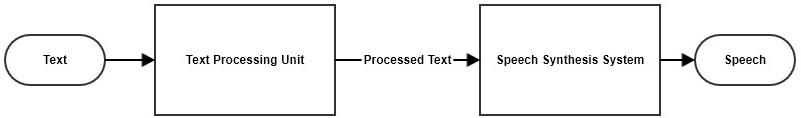
\includegraphics[width=\linewidth]{images/tts_flow_dg.jpg}
  \caption{TTS Sub Modules}
  \label{fig:TTS Sub Modules}
\end{figure}

\section{Text Processing Unit}
Text processing unit is responsible for processing of text before it is sent to speech synthesis system. It finds numbers, dates and time in input data and converts it into format acceptable by speech synthesizer. This module consists of following sub modules.

\begin{enumerate}
  \item Special Character Processor
  \item Semantic Tagger  
  \item Text Generator
  \item Text Formatter 
\end{enumerate}

\subsection{Special Character Processor}

Raw text may contain special characters such as punctuation marks. These characters help to understand context of a word but 
are not converted into sounds. We remove all such characters from text before further processing. 
Another processing which is done is conversion of all arabic numerals like \textarabic{١}, \textarabic{٢} and \textarabic{٣} into their corresponding 
characters like 1, 2 and 3 because it is easy to further process text after it has been converted into same type of numerals.

\subsection{Semantic Tagger}
The purpose of Semantic Tagger is to identify numbers, dates and time from input data and give them proper tags. 
All numbers in input data are converted into arabic numerals of type 1, 2 and 3 in previous step. 
There can be multiple form of numbers, dates and time. These forms are explained below.


\begin{enumerate}    
  \item Dates in following format

  \begin{enumerate}[label=\alph*.]
    \item 12/11/2018 or 12/11/18 with different separators like \enquote{/} or \enquote{-} or \enquote{.}
    \item \texturdu{12 دسمبر 2012}
    \item \texturdu{12 دسمبر}
  \end{enumerate}
  \item Number in following format
  \begin{enumerate}[label=\alph*.]
    \item Whole Numbers such as 123
    \item Floating point numbers such as 12.3
  \end{enumerate}

  \item Time in following format

  \begin{enumerate}[label=\alph*.]
    \item 12:12
    \item 12:12:12
  \end{enumerate}
\end{enumerate}


In table \ref{table:semantic_tagger_regex}, regex used for identification of these numbers, dates and time are shown.

\begin{table}[]
\centering
\resizebox{\textwidth}{!}{%
\begin{tabular}{|c|c|c|}
\hline
\textbf{Regex} & \textbf{Type} & \textbf{Example} \\ \hline
(\textbackslash{}d+(?:\textbackslash{}.\textbackslash{}d+)?) & Integer or Floating point number & 123 or 12.312 \\ \hline
\textbackslash{}d\{1,2\}:\textbackslash{}d\{1,2\}(?::\textbackslash{}d\{1,2\})? & Time with or without seconds & 5:12 or 5:12:10 \\ \hline
\textbackslash{}d\{1,4\}{[}./-{]}\textbackslash{}d\{1,4\}{[}./-{]}\textbackslash{}d\{1,4\} & Date with separator like \enquote{/} or \enquote{-} or \enquote{.} & 12-10-2018 or 12/10/18 \\ \hline
\%s \textbackslash{}d\{4\} & Dates with month name in Urdu. This is checked by replacing \%s with each month name separately. & \texturdu{12 دسمبر} \\ \hline
\end{tabular}%
}
\caption{Regular Expression for Semantic Tagger}
\label{table:semantic_tagger_regex}
\end{table}

\subsection{Text Generator}
Semantic tagger will return all numbers, dates and time from text with each one marked as date/time/number. Text generator part will take each word and generates Urdu text according to its tagging. Each tagged number is handled by specific text converter. These converters are listed below.

\begin{enumerate}
  \item Number to text converter
  \item Date to text converter 
  \item Time to text converter
\end{enumerate}

\subsubsection{Number to Text Converter}
This unit will deal with whole numbers, fractional numbers and decimal numbers. In table \ref{table:no_conversion_example}, example conversions are shown. 

\begin{table}[]
\centering
\begin{tabular}{|c|c|}
\hline
\textbf{Word} & \textbf{Converted Text}                          \\ \hline
123           & \texturdu{ایک سو تئیس}                                     \\ \hline
1231          & \texturdu{ایک ہزار دو سو اکتیس}                            \\ \hline
123.1234      & \texturdu{ایک سو تئیس اعشاریہ ایک دو تین}                   \\ \hline
12345         & \texturdu{بارہ ھزار تین سو پینتالیس}                        \\ \hline
1234567       & \texturdu{بارہ لاکھ چونتیس ھزار پانچ سو ستاسٹھ}             \\ \hline
987654321     & \texturdu{اٹھانوے کروڑ  چھہتر لاکھ   چون ھزار تین سو اکیس}  \\ \hline
143.159874    & \texturdu{ایک سو تینتالیس  اعشاریہ ایک پانچ نو آٹھ سات چار} \\ \hline
\end{tabular}
\caption{Number Conversion example}
\label{table:no_conversion_example}
\end{table}

Different process is performed in order to handle fractional and integer parts of floating point numbers. The algorithm for integral number is described below.

\begin{minted}[mathescape,
               breaklines, 
               numbersep=5pt,
               gobble=1,
               frame=lines,
               framesep=1mm]{python}
  def get_factors(number):
    factored_integer_list = [100000000000, 1000000000, 10000000, 100000, 1000, 100]
    factored_number = []
    for factor in factored_integer_list:
        If factor > number and number != 0:
            factored_number.append(number/factor)
            factored_number.append(factor)
            number = number % factor  
    If number != 0:
        factored_number.append(number)
    return factored_number

\end{minted}

This algo will return list of factored numbers and factors. For 1213, the result of this algorithm will be 
[1, 1000, 2, 100, 13]. The integer to Urdu mapping for number 0 to 100 and number like 1000, 100000 etc are 
stored in CSV file. The factored number list will then be converted into text by using integer to Urdu mapping. 
In table \ref{table:number_mapping}, Urdu mapping of each possible factor is listed. Each number in fractional 
part of floating pointing number is replaced by their respective mapping from above list. 
Both the mappings of integral and fractional part of number are then joined to get
complete text of input number. This module is very important module as it is also used in date and time conversion.  

\subsubsection{Date to Text Converter}

The unit deals with date in following formats

\begin{itemize}
  \item 12/12/2012
  \item 12/12/12
  \item 12.12.2012
  \item 12.12.12
  \item 12-12-2012
  \item 12-12-12
  \item \texturdu{12 دسمبر 2012}
\end{enumerate}

All dates will be converted into common format e.g. \texturdu{ بارہ دسمبر دو ہزار بارہ}. Some example conversions are shown in table \ref{table:example_of_date_conversions}.

\begin{table}[]
\centering
\begin{tabular}{|c|c|}
\hline
\textbf{Date} & \textbf{Converted Text}            \\ \hline
12/10/15      & \texturdu{دس دسمبر  دو ھزار پندرہ} \\ \hline
12.10.15      & \texturdu{دس دسمبر  دو ھزار پندرہ} \\ \hline
12-10-15      & \texturdu{دس دسمبر  دو ھزار پندرہ} \\ \hline
12.10.1989    & \texturdu{دس دسمبر انیس سو نواسی}  \\ \hline
\end{tabular}
\caption{Example Date Conversions}
\label{table:example_of_date_conversions}
\end{table}

The word tagged as date is first processed to get year, month and day of the month. Day and year are then passed to number to text converter and month is 
converted to its corresponding mapping. This mapping is saved in CSV file. This is shown in table \ref{table:month_mapping}. 
In Urdu, in dates, we have different notation for year e.g. 1980 in number is spoken as \texturdu{ایک ھزار نو سو نواسی} (One thousand nine hundred and 
eighty nine) but in dates, it is spoken as \texturdu{انیس سو نواسی} 
(Nineteen hundred and eighty nine). This is also handled during the process of date to text conversion.


\subsubsection{Time to Text Converter}

Time can occur with seconds or without seconds in text. It is written in 1:11:12 or 1:12 format. All words tagged as time will be converted into text 
by separating hour, minutes and seconds from time. Each value will be converted into Urdu text by using number to text converter. All these values are 
combined to make complete time text. Table \ref{table:example_time_conversion} shows example conversions.

\begin{table}[]
\centering
\begin{tabular}{|c|c|}
\hline
\textbf{Time} & \textbf{Converted Text}                        \\ \hline
1:12:15       & \texturdu{ایک بج کر  بارہ منٹ اور پندرہ سیکنڈ} \\ \hline
7:45          & \texturdu{سات بج کر پینتالیس منٹ}              \\ \hline
\end{tabular}
\caption{Example Time Conversions}
\label{table:example_time_conversion}
\end{table}

\subsection{Text Formatter}
The purpose of formatter is to replace all number, dates and time with their corresponding Urdu text returned by Text generator. 
This process is performed in following order
\begin{enumerate}
  \item Word tagged as dates are replaced by their corresponding text
  \item Word tagged as time are replaced by their corresponding text
  \item Word tagged as number are replaced by their corresponding text. 
\end{enumerate}
The output of all above processes will be the text which will only contain Urdu text which can now pass to the speech synthesizer which will convert it to speech signals. 

\section{Speech Synthesis System}

\subsection{Tools}

Below are the tools used for the process of Speech Synthesis of Urdu.

\begin{enumerate}
  \item Speech Tools Library of Edinburg
  \item Festvox
  \item Speech Signal Processing Toolkit (SPTK)
  \item Festival
\end{enumerate}

\subsubsection{Speech Tools Library of Edinburg}
The Edinburgh Speech tools is collection of utilities used for speech processing. These utilities cover major tasks such that reading and 
writing speech waveforms, parameter files(F0 and LPC etc). The speech tools also include executable programs which can 
be used in user defined programs.


\subsubsection{Festvox}
Festvox is a tool which can be used to build synthetic voices. This includes scripts for building voice in other languages.

\subsubsection{ Speech Signal Processing Toolkit (SPTK)}
As name suggests, this tool is for processing speech signals in UNIX systems. 

\subsubsection{Festival}

Festival \cite{thefestivalspeechsynthesissystem} is a speech synthesis system which is developed in Centre for Speech Technology Research (CSTR) \cite{centreforspeechtechnologyresearch}. It is a multi-platform framework for building speech synthesis system. This system is outlined so that it tends to be utilized for following purposes

\begin{enumerate}
  \item Improvement in speech synthesis system
  \item Developing speech synthesis applications
\end{enumerate}

One of the main thing that makes Festival very useful is scripting language which is based upon Scheme programming language. This can be used to manage parameters and flow of  control in Festival. 

\subsection{Process}

The process of speech synthesis is based on statistical parametric speech synthesis. The statistical parametric speech synthesis system is based on models like HMM or DNN in which recorded speech is used to train model. In this method, speech is elaborated with parameters which are defined by statistics. This is why it is called as statistical parametric speech synthesis. 

In CLUSTERGEN statistical parametric speech synthesis, model is trained and used for synthesis in Festival Speech Synthesis system. 

\subsubsection{Preparing Data}

For training purpose, Phonetically Rich Urdu Speech Corpus \cite{urdu_corpus} is used. This data consists of recordings of 708 phonetically rich sentences, 
10,101 tokens with 5,656 unique words. Total duration of recording is 70 minutes.

\subsubsection{Data Labeling}
Data is labeled in specific format which is required by FestVox for training purpose. The is labeled in following format.
\\ \\
( c1 "\texturdu{نیلم نے سالگرہ پر ہیڈ سیسموگراف اسود قریشی کے ماتھے پر اینٹھن اور غم کی آتشیں رو محسوس کی}" )

Where c1 is the name of recording file and text between quotation marks is corresponding label of that recording.

\subsubsection{Training Data}

The whole data is further divided in 10:1 ratio in training and test set respectively.


\subsubsection{Urdu to Hindi Transliteration}

The underlying system of Urdu TTS is Hindi TTS system. So all the alphabets are mapped in their corresponding Hindi alphabets. 
In this way, text is first converted into corresponding Hindi text using that mapping and then it is converted into sound. 
Mapping of each Urdu word with Hindi in this system is shown in table \ref{table:hindi_to_urdu}.

\subsubsection{Data Labeling}

The first stage of training is to label speech database using HMM labeler. We are using EHMM labeler which is provided in FestVox. In this process, Baum-Welch is used to train context dependent models. This labeler works in 8 steps. Prompt files are extracted from utterance structure of Festival.

\begin{itemize}
  \item Unique sequence of phones are extracted and stored.
  \item List of wav files is collected for feature extraction.
  \item From wav files, cepstral coefficients (LPCCs and MFCCs) are extracted.
  \item From cepstral coefficients, deltas and delta-delta features are generated.
  \item By using generated features and wav files list, features vectors are modified.
  \item Phones list generated in step # 2 and wav file list is used to modify prompt list.
  \item Hidden Markov model is trained using Baum-Welsh algorithm till difference in the average likelihood is less than 0.001.
  \item Labels are generated according to training data.
  \item Integer indices of labels are converted into phone names
\end{enumerate}

\subsubsection{Building Utterance Structure}

Utterance is the essential building unit of Festival. It shows relation between bunch of items where each item relates to word, syllable or segment etc. Below are the some of the relations used in building utterance structure.

\begin{itemize}
  \item{\textbf{Text}:} It consists of strings to be processed and features of that string.
  \item{\textbf{Token}:} Token means each word in a sentence is separated by some language specific separator.
  \item{\textbf{Word}:} A small unit of speech which can be pronounced with the help of letter to sound rules of a language.
  \item{\textbf{Phrase}:} Phrase means group of words forming a part of a sentence.
  \item{\textbf{Syllable}:} Syllables are units which when combined with vowels form complete pronunciation of a word.
  \item{\textbf{Segment}:} Segment consists of list of phones.
  \item{\textbf{SylStructure}:} This is a tree structure which is formed with word, syllable and segment.
  \item{\textbf{IntEvent}:} These are array of syllable related intonation events.
  \item{\textbf{Intonation}:} Intonation means rise and fall in speech signals.
\end{itemize}


\subsubsection{Coefficient Extraction}
Coefficient extraction is the process of extracting parameters like F0, mcep and voicing coefficients using SPTK. This is done by 
generating F0 and mcep coefficient. These parameters are then combined to make final parameter files. 
This is a lengthy process which can take lot of time depending on size of training data.

\subsubsection{Building the Model}

All the data generated above is used to train and build HMM-state duration model. This process works in following steps.

\begin{enumerate}
  \item Statenames Generation
  \item Parametric Model generation
  \item Duration model generation for statenames
\end{enumerate}

This resulting model can be used to perform TTS synthesis process.

\appendix
\chapter{Figures}

\vspace*{-3in}

\begin{figure}
\vspace{2.4in}
\caption{Armadillo slaying lawyer.}
\label{arm:fig1}
\end{figure}
\clearpage
\newpage

\begin{figure}
\vspace{2.4in}
\caption{Armadillo eradicating national debt.}
\label{arm:fig2}
\end{figure}
\clearpage
\newpage

\chapter{Tables}

\begin{longtable}[c]{|c|c|}
\hline
\textbf{Number} & \textbf{Mapping}    \\ \hline
\endhead
%
.               & \texturdu{اعشاریہ}  \\ \hline
0               & \texturdu{زیرو}     \\ \hline
1               & \texturdu{ایک}      \\ \hline
2               & \texturdu{دو}       \\ \hline
3               & \texturdu{تین}      \\ \hline
4               & \texturdu{چار}      \\ \hline
5               & \texturdu{پانچ}     \\ \hline
6               & \texturdu{چھ}       \\ \hline
7               & \texturdu{سات}      \\ \hline
8               & \texturdu{آٹھ}      \\ \hline
9               & \texturdu{نو}       \\ \hline
10              & \texturdu{دس}       \\ \hline
11              & \texturdu{گیارہ}    \\ \hline
12              & \texturdu{بارہ}     \\ \hline
13              & \texturdu{تیرہ}     \\ \hline
14              & \texturdu{چودہ}     \\ \hline
15              & \texturdu{پندرہ}    \\ \hline
16              & \texturdu{سولہ}     \\ \hline
17              & \texturdu{سترہ}     \\ \hline
18              & \texturdu{اٹھارہ}   \\ \hline
19              & \texturdu{انیس}     \\ \hline
20              & \texturdu{بیس}      \\ \hline
21              & \texturdu{اکیس}     \\ \hline
22              & \texturdu{بائیس}    \\ \hline
23              & \texturdu{تئیس}     \\ \hline
24              & \texturdu{چوبیس}    \\ \hline
25              & \texturdu{پچیس}     \\ \hline
26              & \texturdu{چھبیس}    \\ \hline
27              & \texturdu{ستائیس}   \\ \hline
28              & \texturdu{اٹھائیس}  \\ \hline
29              & \texturdu{انتیس}    \\ \hline
30              & \texturdu{تیس}      \\ \hline
31              & \texturdu{اکتیس}    \\ \hline
32              & \texturdu{بتیس}     \\ \hline
33              & \texturdu{تینتیس}   \\ \hline
34              & \texturdu{چونتیس}   \\ \hline
35              & \texturdu{پینتیس}   \\ \hline
36              & \texturdu{چھتیس}    \\ \hline
37              & \texturdu{سینتیس}   \\ \hline
38              & \texturdu{اٹھتیس}   \\ \hline
39              & \texturdu{انتالیس}  \\ \hline
40              & \texturdu{چالیس}    \\ \hline
41              & \texturdu{اکتالیس}  \\ \hline
42              & \texturdu{بیالیس}   \\ \hline
43              & \texturdu{تینتالیس} \\ \hline
44              & \texturdu{چوالیس}   \\ \hline
45              & \texturdu{پینتالیس} \\ \hline
46              & \texturdu{چھیالیس}  \\ \hline
47              & \texturdu{سینتالیس} \\ \hline
48              & \texturdu{اڑتالیس}  \\ \hline
49              & \texturdu{انچاس}    \\ \hline
50              & \texturdu{پچاس}     \\ \hline
51              & \texturdu{اکیاون}   \\ \hline
52              & \texturdu{باون}     \\ \hline
53              & \texturdu{تریپن}    \\ \hline
54              & \texturdu{چون}      \\ \hline
55              & \texturdu{پچپن}     \\ \hline
56              & \texturdu{چھپن}     \\ \hline
57              & \texturdu{ستاون}    \\ \hline
58              & \texturdu{اٹھاون}   \\ \hline
59              & \texturdu{انسٹھ}    \\ \hline
60              & \texturdu{ساٹھ}     \\ \hline
61              & \texturdu{اکسٹھ}    \\ \hline
62              & \texturdu{باسٹھ}    \\ \hline
63              & \texturdu{تریسٹھ}   \\ \hline
64              & \texturdu{چونسٹھ }  \\ \hline
65              & \texturdu{پینسٹھ}   \\ \hline
66              & \texturdu{چھیاسٹھ}  \\ \hline
67              & \texturdu{ستاسٹھ}   \\ \hline
68              & \texturdu{اٹھاسٹھ}  \\ \hline
69              & \texturdu{انهتر}    \\ \hline
70              & \texturdu{ستر}      \\ \hline
71              & \texturdu{اکھتر}    \\ \hline
72              & \texturdu{بھتر}     \\ \hline
73              & \texturdu{تھتر}     \\ \hline
74              & \texturdu{چوہتر}    \\ \hline
75              & \texturdu{پچھتر}    \\ \hline
76              & \texturdu{چھہتر}    \\ \hline
77              & \texturdu{ستتر}     \\ \hline
78              & \texturdu{اٹھتر}    \\ \hline
79              & \texturdu{اناسی}    \\ \hline
80              & \texturdu{اسی}      \\ \hline
81              & \texturdu{اکاسی}    \\ \hline
82              & \texturdu{بیاسی}    \\ \hline
83              & \texturdu{تراسی}    \\ \hline
84              & \texturdu{چوراسی}   \\ \hline
85              & \texturdu{پچاسی}   \\ \hline
86              & \texturdu{چھیاسی}   \\ \hline
87              & \texturdu{ستاسی}    \\ \hline
88              & \texturdu{اٹھاسی}   \\ \hline
89              & \texturdu{نواسی}    \\ \hline
90              & \texturdu{نوے}      \\ \hline
91              & \texturdu{اکانوے}   \\ \hline
92              & \texturdu{بانوے}    \\ \hline
93              & \texturdu{ترانوے}   \\ \hline
94              & \texturdu{چورانوے}  \\ \hline
95              & \texturdu{پچانوے}   \\ \hline
96              & \texturdu{چھیانوے}  \\ \hline
97              & \texturdu{ستانوے}   \\ \hline
98              & \texturdu{اٹھانوے}  \\ \hline
99              & \texturdu{ننانوے}   \\ \hline
100             & \texturdu{سو}       \\ \hline
1000            & \texturdu{ھزار}     \\ \hline
100000          & \texturdu{لاکھ  }   \\ \hline
10000000        & \texturdu{کروڑ }    \\ \hline
1000000000      & \texturdu{ارب }     \\ \hline
100000000000    & \texturdu{کھرب }    \\ \hline
\caption{Number Mappings}
\label{table:number_mapping}\\
\end{longtable} 

\begin{longtable}[c]{|c|c|}
\hline
\textbf{Number} & \texturdu{\textbf{Mapping}} \\ \hline
\endhead
%
january         & \texturdu{جنوری}            \\ \hline
february        & \texturdu{فروری }           \\ \hline
march           & \texturdu{مارچ }            \\ \hline
april           & \texturdu{اپریل}            \\ \hline
may             & \texturdu{مئی}              \\ \hline
june            & \texturdu{جون }             \\ \hline
july            & \texturdu{جولائی}           \\ \hline
august          & \texturdu{اگست}             \\ \hline
september       & \texturdu{ستمبر }           \\ \hline
october         & \texturdu{اکتوبر }          \\ \hline
november        & \texturdu{نومبر }           \\ \hline
december        & \texturdu{دسمبر}            \\ \hline
1               & \texturdu{جنوری}            \\ \hline
2               & \texturdu{فروری }           \\ \hline
3               & \texturdu{مارچ }            \\ \hline
4               & \texturdu{اپریل}            \\ \hline
5               & \texturdu{مئی}              \\ \hline
6               & \texturdu{جون }             \\ \hline
7               & \texturdu{جولائی}           \\ \hline
8               & \texturdu{اگست}             \\ \hline
9               & \texturdu{ستمبر }           \\ \hline
10              & \texturdu{اکتوبر }          \\ \hline
11              & \texturdu{نومبر }           \\ \hline
12              & \texturdu{دسمبر}            \\ \hline
\caption{Month Mapping}
\label{table:month_mapping}
\end{longtable}

\nocite{*}
\printbibliography

\end{document}
